


  If $\overline{AB}$ (not drawn) is a diameter of a semicircle, then what is the area of the region below in terms of $x$?
\begin{center}
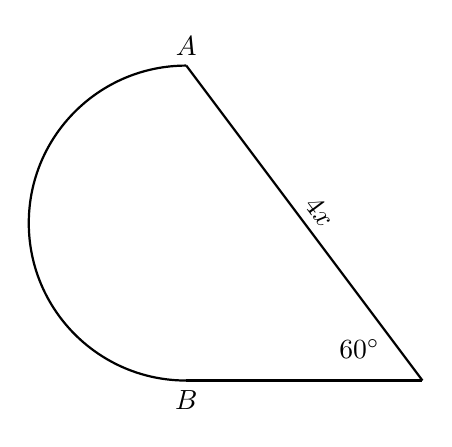
\begin{tikzpicture}
    \draw[thick] (0,2) arc (90:270:2);
   
    \draw[thick] (0,2)--(3,-2) node[above, midway, sloped]{$4x$};
    \draw[thick] (0,-2)--(3,-2);
    \draw node at (2.2,-1.6) {$60^\circ$};    
    \draw node[above] at (0,2) {$A$};         
    \draw node[below] at (0,-2) {$B$};               
       
               
\end{tikzpicture} 
\end{center}



\ifsat
	\begin{enumerate}[label=\Alph*)]
		\item   $1.5x^{2}\pi+2x^{2}\sqrt{3}$ %
		\item  $3x^{2}\pi+2x^{2}\sqrt{3}$
		\item  $1.5x^{2}\pi+4x^{2}\sqrt{3}$ 
		\item  $3x^{2}\pi+8x^{2}\sqrt{3}$
	\end{enumerate}
\else
\fi

\ifacteven
	\begin{enumerate}[label=\textbf{\Alph*.},itemsep=\fill,align=left]
		\setcounter{enumii}{5}
		\item   $1.5x^{2}\pi+2x^{2}\sqrt{3}$ %
		\item  $3x^{2}\pi+2x^{2}\sqrt{3}$
		\item  $1.5x^{2}\pi+4x^{2}\sqrt{3}$ 
		\addtocounter{enumii}{1}
		\item  $3x^{2}\pi+4x^{2}\sqrt{3}$
		\item  $3x^{2}\pi+8x^{2}\sqrt{3}$
	\end{enumerate}
\else
\fi

\ifactodd
	\begin{enumerate}[label=\textbf{\Alph*.},itemsep=\fill,align=left]
		\item   $1.5x^{2}\pi+2x^{2}\sqrt{3}$ %
		\item  $3x^{2}\pi+2x^{2}\sqrt{3}$
		\item  $1.5x^{2}\pi+4x^{2}\sqrt{3}$ 
		\item  $3x^{2}\pi+4x^{2}\sqrt{3}$
		\item  $3x^{2}\pi+8x^{2}\sqrt{3}$
	\end{enumerate}
\else
\fi

\ifgridin
   $1.5x^{2}\pi+2x^{2}\sqrt{3}$ %
		
\else
\fi

